\documentclass[runningheads]{llncs}
%
\usepackage{algorithm}
\usepackage{amsmath}
\usepackage{amssymb}
\usepackage{algpseudocode}
\usepackage{graphicx}
% Used for displaying a sample figure. If possible, figure files should
% be included in EPS format.
%
% If you use the hyperref package, please uncomment the following line
% to display URLs in blue roman font according to Springer's eBook style:

%\hypersetup{
%   colorlinks=false,
%  pdfborder={0 0 0},
%}
\usepackage{hyperref,xcolor}% http://ctan.org/pkg/{hyperref,xcolor}
\usepackage{makeidx}
\definecolor{winered}{rgb}{0.5,0,0}
  
\hypersetup
{
    pdfauthor={Anurag Dutta},
    pdfsubject={Hyperlinks in LaTeX},
    pdftitle={myhyper.tex},
    pdfkeywords={LaTeX, PDF, hyperlinks}
%    colorlinks=false,
    pdfborder={0 0 0},
%You can set individual colors for links as below:
colorlinks=true,
 linkcolor=winered,
urlcolor={winered},
filecolor={winered},
%citecolor={winered} %Gives errors when turned on
%allcolors={winered} %Gives errors when turned on
  linktoc=all,
}
\begin{document}
%
\title{Predicting Steam Games review vis-à-vis ChaosNet}
%
%\titlerunning{Abbreviated paper title}
% If the paper title is too long for the running head, you can set
% an abbreviated paper title here
%
\author{Anurag Dutta\inst{1}\orcidID{0000–0002–5787–3860}}
%
\authorrunning{A. Dutta}
% First names are abbreviated in the running head.
% If there are more than two authors, 'et al.' is used.
%
\institute{Undergraduate, Department of Computer Science and Engineering, Government College of Engineering and Textile Technology, Serampore, Calcutta, India \\\textbf{\\}
\email{anuragdutta.research@gmail.com}\\
}
%
\maketitle              % typeset the header of the contribution
%
\begin{abstract}
Video games, often known as computer games, are digital games that use a graphical user interface or input device, such as a joystick, console, keyboard, or motion sensor array, to create sensory feedback. This input is typically exhibited on a visual display device, such as a TV, monitor, touchpad, or virtual reality headset. Some video games, like text adventures and computer chess, which utilise teletype printers, can be played without a visual display. Gaming audio feedback through speakers or headphones is a popular addition. There are also sporadic uses for other types of feedback, such as haptic technologies. The digital game retail and distribution service "Steam" is provided by Valve. Programmers can integrate Steamworks, a free programming interface for applications (API), into their works to support features like in-game achievements, microtransactions, and user-generated content. This API was introduced by Valve in 2008. In 2010 and 2012, respectively, Steam was first made available for the macOS and Linux operating systems. We have collected details about a total of 36608 Titles from Steam Officials. Following the same, we have intrinsic information regarding "Name of the Titles", "Initial Price of the Release", "Discounted Price of the Release", "Windows Platform Support Available or not?", "Mac Platform Support Available or not?", "Linux Platform Support Available or not?", and the "Reviews" subjected to these features. In this work, we would try to build a model to predict the Reviews of different titles provided their intrinsic features. For that, we would make use of ChaosNet - an Artificial Neural Network constructed using Generalized Luroth Series maps. Objectively, Chaos has been identified in the brain at several spatiotemporal scales. Numerous neural models, such as the Hindmarsh-Rose neuron model, reveal complex chaotic dynamics, and it is known that individual brain neurons exhibit chaotic bursting activity. Although many Artificial Neural Networks (ANNs), including Recurrent Neural Networks, involve Chaos, there isn't an Artificial Neural Network for classical tasks that is entirely composed of Chaos. With cutting-edge accuracy in the small training sample pool, ChaosNet solves classification problems using the topological transitivity property of chaotic GLS neurons. By learning from a small set of training data, this network can complete categorization tasks.
\keywords{Video Games \and Steam \and Game Reviews \and ChaosNet \and Artificial Neural Network}
\end{abstract}
%
%
%
\section{Introduction}
Learning using methodologies like Machine Learning (ML) \& Deep Learning (DL) has become popular due to the development of Artificial Intelligence and has applications in almost every field of human endeavour. Voice processing, computer vision, information security, and clinical diagnosis are just a few examples of these. The cognitive and memory imprinting mechanisms in humans are not closely attached to these algorithms, although being guided by the biological brain. The weights and biases of these artificial neural networks (ANNs) are changed through earning procedures that rely on optimization techniques and the minimization of loss or error functions. The ANNs now use an enormous number of fixed hyperparameters remedied via an ad hoc technique for better prediction as more and more new data is fed into the system. These synaptic changes are mostly based on empirical data and lack or have weak theoretical underpinnings. Additionally, for these techniques to accurately predict or categorise the distribution of the target classes, a large amount of training data is required.\\

Although ANNs have made significant progress, they still lag far behind human intelligence in applications like natural language processing. In order to take advantage of the human brain's extraordinary capacity for learning and to gain a deeper understanding of the brain, researchers are focusing on developing biologically inspired algorithms and architectures. In terms of memory encoding and learning, this is being done. One of the most fascinating characteristics of the brain is its ability to exhibit "Chaos," the phenomenon in which simple deterministic nonlinear systems display complicated unexpected and random-like behaviour. It is well known that electroencephalogram (EEG) data have chaotic dynamics. The ability of a brain system to respond optimally to multiple influences is facilitated by its sensitivity to minute changes in internal operating features. This characteristic is similar to the dynamical properties of chaotic systems. It is also clear that the brain does not return to equilibrium after a transient but rather alternates between a number of states continuously. Because of this, it is theorised that the brain, depending on the functional characteristics of the neurons, can exhibit a range of behaviours, such as periodic orbits, weak chaos, and strong chaos. Chaotic activity can be seen in brain networks, which are composed of billions of neurons, as well as in the cellular and subcellular dynamics of individual neurons. The brain can transfer and store information thanks to these neurons' capacity to create impulse trains. Action potentials or impulses are created when different ions penetrate the axonal membrane and alter the voltage across it. Hodgkin and Huxley were the first to propose a dynamical system's model for the interaction between the ion channels and the axon membrane that can generate precise action potentials. Later, it was suggested to employ its more simplified equivalents, like the Hindmarsh-Rose model and the Fitzugh-Nagumo model. All of these models exhibit disorderly behaviour. We were unaware of any architectures described thus far for classification tasks that exhibit chaos at the level of individual neurons, despite the fact that recurrent neural networks are one type of artificial neural network that exhibits chaotic dynamics. Other chaotic neuron theories, on the other hand, have been put out as a possible theoretical justification for memory encoding in the brain.\textbf{\\}

The Aihara model, one of these models, has been used to study cognitive activities in the network's unpredictable periodic orbits. In order to illustrate how odours are remembered, Freeman, Kozma, and colleagues created chaotic simulators that were inspired by the mammalian sensorimotor pathway. Tsuda and others have also investigated chaos in neural networks. Kaneko investigated the dynamical features of globally coupled chaotic maps and proposed that these networks may manage biological data. \textbf{\\}

An artificial neural network called \textit{\textbf{ChaosNet}} is composed of 1D chaotic map neurons of the Generalized Luröth Series (GLS). For classification tasks, this network can learn from a limited amount of training instances. ChaosNet was created to make use of some of the most advantageous features of biological neural networks. It has been shown that it can perform challenging classification tasks on par with or better than classic ANNs while using much less training samples than traditional ANNs. A "spike-count rate"-like characteristic of the flashing of chaotic neurons is used by ChaosNet, which again was inspired by real neurons, as a neural code for training. A hierarchical architecture may also be present in the network, including data as it is sent to deeper, higher layers of the network. The neuron that we propose is represented by a variational linear 1D chaotic map called the generalised Luröth series, or GLS. The well-known Tent map, Binary map, and its skewed relatives are examples of GLS. Figure \ref{fig1} shows the Architecture behind ChaosNet. The types of GLS neurons used in ChaosNet include 
\begin{equation}
T_{Skew-Binary}(x)=\left\{\begin{matrix}\frac{x}{b}&0\le x<b\\\frac{\left(x-b\right)}{\left(1-b\right)}&b\le x<1\\\end{matrix}\right.
\end{equation}
and
\begin{equation}
T_{Skew-Tent}(x)=\left\{\begin{matrix}\frac{x}{b}&0\le x<b\\\frac{\left(1-b\right)}{\left(1-b\right)}&b\le x<1\\\end{matrix}\right.
\end{equation}
where, $b$ is the Skew Parameter.
\begin{figure}
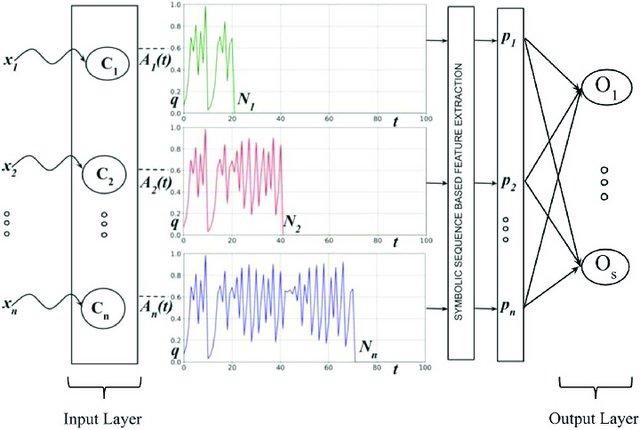
\includegraphics[width=\textwidth]{1.jpg}
\caption{ChaosNet's architecture consists of Generalized Luroth neural networks for classification-related tasks. The unit dimensional GLS neurons are designated as $C_1$, $C_2$,..., $C_n$. At first, each neuron displays q units of typical neural activity. The symbol $\left\{x_i\right\}_{i=1}^n$ designates the input to the network, or the normalised collection of stimuli. Starting with the initial neuronal activity ($q$), a GLS neuron's chaotic activity value $A_i(t)$ increases until it reaches the vicinity of the stimulus, at which point it ceases to fire chaotically. The firing time of this neuron is $N_i$ ms. Topological transitivity symbolic sequence characteristic pi is present in $A_i(t)$. This characteristic is taken from the GLS-neuron of the $C_i$, $A_i(t)$.} \label{fig1}
\end{figure}
\\\\A rapidly expanding application genre is video games. Since the game business generated \$180 billion in sales in 2021, it is anticipated that PC gaming will expand to \$268 by 2025. However, creating a successful game is difficult due to the size of the computer gaming business. Additionally, previous research has demonstrated that gamers are a set of people that are very challenging to please, making the calibre of games a significant concern. Game creators must have a deeper grasp of players' problems in order to increase the user-perceived quality of their games. The majority of current research on game quality, however, has concentrated on developer-perspective quality issues, while just a small number of studies have addressed specific user-perspective difficulties. Many online game distribution platforms permit users to publish evaluations of a game, just like mobile app distribution platforms like the Apple App Store and Google Play do. These game reviews offer a comprehensive data source that can be used to comprehend user-reported problems better. The importance of reviewing reviews has been demonstrated in previous work on mobile apps. \textbf{\\}

In this research, we analyse 36,869 game reviews from the Steam platform, one of the most well-liked digital game distribution platforms, in order to gain a deeper understanding of the user-reported game concerns. Based on its inherent values, such as Actual Price, Discounted Price, and Support for many platforms, our purpose is to comprehend and foretell the reviews of each recently launched title. Thus, this knowledge will aid game producers in better understanding how to use user reviews to raise the perceived quality of their games among players. Additionally, our work may serve as a springboard for longer-term studies of game reviews and may suggest fresh avenues for further investigation.
\section{Steam}
The Valve Corporation created the digital game distribution system known as Steam. Prior to the 1998 release of Half-Life, Valve and Sierra Studios had a publishing agreement. Along with publishing authority, Sierra was also granted some intellectual property (IP) rights under the deal. Through Sierra, Valve released other titles, including Half-Life and Counter-Strike expansions. Around 1999, as Valve began developing Half-Life 2 and the new Source engine, they started to worry about their agreement with Sierra over IP rights. By 2001, the two businesses had negotiated a new agreement. The new agreement granted Valve control over the digital distribution of Sierra's games while removing Sierra's IP rights. Since giving downloading patches for multiplayer games resulted in the majority of the online user base disconnecting for several days until players had installed the patch, Valve was seeking for a better way to update its published titles. Valve made the decision to develop a platform that would automatically update games and put more effective anti-cheat and anti-piracy safeguards in place. In addition, Valve recognised that they could deliver game content to players more quickly than through retail channels at the time of its 2002 announcement because at least 75\% of their users had access to high-speed Internet connections, a number that would increase with planned broadband expansion in the coming years. The platform's initial working names, "Grid" and "Gazelle," were used when development on Steam started in 2002. On March 22, 2002, it was made public during a GDC event and made available for beta testing the following day. Relic Entertainment developed a special edition of Impossible Creatures in order to show how simple it is to integrate Steam with a game. Acer, GameSpy, AT\&T, and other businesses joined forces with Valve. Day of Defeat was the initial mod made available for the platform. Gabe Newell, the president of Valve, declared in 2002 that he was prepared to sell mod teams on a game engine licence and Steam distribution for \$999. Through 2002, Valve filed a lawsuit against Sierra and its owners, Vivendi Games, after discovering that Sierra had been distributing its games in PC cafes, in violation of the terms of their contract, prior to the launch of Steam. With the launch of Steam, Sierra countersued, alleging that Valve had been attempting to undermine the agreement by providing a digital marketplace for their games in direct competition with Sierra. The lawsuit was first decided in Valve's favour, enabling them to continue working on Steam while terminating the agreement due to the breach and looking for other publishing partners for retail copies of their titles. Microsoft was one of these companies, but Ed Fries claimed that the corporation declined the offer because Valve intended to keep selling its games through Steam. Before the beta test for Steam's official release on September 12, 2003, 80,000 to 300,000 players took part. At debut, the client and website experienced problems and errors. At the time, Steam was an optional feature for all other games, and its main purpose was to streamline the patch procedure typical in online computer games. Any online elements of games that needed the World Opponent Network ceased to function unless they switched to Steam once it was discontinued in 2004. Half-Life 2 was the first game to be made available digitally on Steam in November 2004 and required the Steam software to be installed in order to play for retail versions. Users encountered difficulties while attempting to play the game at this time. Concerns concerning software ownership, programme specifications, and the Counter-Strike rollout's previous server overload issues were raised in response to the demand of Steam. 2005 saw the hiring of independent game developers to create titles like Rag Doll Kung Fu and Darwinia for the Steam platform. Because of certain very popular Valve games, Valve said that Steam was now profitable. Although retail volume could not yet be matched by digital distribution, Steam offered much higher profit margins for Valve and developers. In 2007, game publishers like id Software, Eidos Interactive, and Capcom started selling their titles on Steam. 13 million accounts had been formed on the service by May of that year, and 150 games were available for purchase. More game publishers joined the service in 2008, including Ubisoft, THQ, Sega, Take-Two Interactive, Activision, and Electronic Arts, but certain titles were either not available or too expensive for markets outside of North America. A free Steam copy of Half-Life 2: Lost Coast and Half-Life 2: Deathmatch was made available to ATI Radeon owners in May 2007, and Steam was also incorporated into the ATI Catalyst GPU driver. Nvidia advertised Steam in the Nvidia GPU driver in January 2008 and gave Nvidia hardware owners a free Steam copy of Portal: The First Slice. For example, Call of Duty: Modern Warfare 2 from Activision in 2009, Fallout: New Vegas from Bethesda Softworks in 2010, and Dragon Age II from Electronic Arts in 2011 all required the installation of Steam. Due to stringent terms of service, Electronic Arts withdrew some of its games off Steam in 2011 and released Mass Effect 3 exclusively through its Origin service in 2012. According to Newell, "We have to prove to EA that having EA titles on Steam is a wise option, and we're going to try to prove that." Ubisoft titles began requiring Uplay to run after being started from Steam in 2014. Due to Valve's refusal to alter its revenue sharing scheme, Ubisoft was unable to sell Tom Clancy's The Division 2 on Steam in 2019. However, it was still available on Uplay and the Epic Games Store. Microsoft began selling its games on Steam in May 2019 in addition to the Microsoft Store. In 2020, EA began publishing a few games on Steam and launching their newly renamed subscription service, EA Play. Around \$1.5 billion in annual video game sales were thought to have been achieved on Steam by 2014. The service had approximately 90 million active monthly users by 2018. In comparison to fewer than 4 billion in 2014, its network transmitted 15 billion gigabytes of data in 2018. Currently, with over 8,000 titles accessible and over 184 million active users, Steam is one of the biggest digital distribution platforms for PC gaming. Steam delivers multiplayer gaming, social networking, and digital rights management (DRM) through its two main platform elements, the Steam Store and the Steam Community. The Steam Store allows users to buy games. A user can play games after logging in to Steam using the Steam client, including games bought through the Steam Store and games bought from third-party vendors and then licensed through the Steam platform. The Steam client will check who owns the game and will download and instal any updates that are readily available. To play a game through Steam, you must first apply the most recent update. Additionally, users can benefit from social network-type services like acquaintances networks through the Steam Forum. On so-called channels, game developers and broadcasters can post news updates for games. In general, although it is not required, developers frequently do send latest information about their games to one or more channels to notify players of the most recent information about their games. After playing a game, players are also able to publish reviews in the Steam Community. Instead of using a 5-star rating system like other well-known platforms for application distribution, players are requested to express how they feel about the game overall by selecting either "Recommended" or "Not Recomended". Alongside the review, information such as the amount of hours spent playing the reviewed game, the total number of games played, and the total number of reviews the reviewer has previously posted are displayed. Developers must go through a tax and identification verification process, pay a \$100 product submission fee for each game, then publish it in the Steam Store. Additionally, the game must go through review phases during which members of the Steam staff play each game to ensure that it is configured correctly, matches the information on the store page, and is free of dangerous code. The quality of the games that are offered on the Steam Store is ensured by the rigorous publication process for games on the Steam Platform. Similar review procedures may be found in mobile app shops like the Apple App Store and the Google Play Store. But unlike Google Play, which has a one-time membership fee of \$25, or the Apple App Store, which charges a \$99 yearly developer membership fee, Steam charges a fee for each product submission. 
\section{Dataset}
The Dataset have been gathered from official sources. It contains details of a total of 36608 Titles. The Features covered in the set are, Actual Price, that is the price of the Game at the time of release. Many time, the releasing brand gives a discount on the price of the product to increase their sales. The dataset also got it covered. It also have the discounted price for each and every titles. Further, as we know, the games are nothing but a chunk of developmental piece of code, so they needs constant maintenance. The maintenance is sometimes not available for some Operating System. Like, these games now a day are targeted towards 3 platforms, Windows, Mac, and Linux. If any title fails to give support for any of these platforms, the dataset have also got it covered. The Labels for each Title, have also been entitled. The labels being Positive(2), Mixed(1), and Negative(0). The dataset have been made available at \href{https://github.com/Anurag-Dutta/Predicting-Steam-Games-review-vis---vis-ChaosNet-/blob/main/SteamDataset.csv}{https://github.com/Anurag-Dutta/Predicting-Steam-Games-review-vis---vis-ChaosNet-/blob/main/SteamDataset.csv}. 
\section{Results}
The Problem of Prediction is subjected to Classification, and hence it gives a clear indication that we can make use of the Classification Algorithms. For each of these algorithms, we made use of specifically 2 metrics for our job - Training F1 Score, and Testing F1 Score. One more point to note hereby in our work is that, the F1 Score, that we would be using in our work ins the Macro F1 Score. The greatest and worst values of the F1 score are 1 and 0, respectively, and it can be thought of as a harmonic mean of recall and precision. Precision and recall are equally represented in the F1 score; "macro" calculates the metrics for each label and determines their unweighted mean. Label imbalance is not taken into consideration in this. The confusion matrix is used to calculate this measure. Mathematically, 
\begin{equation*}
Macro\ F1\ Score\ =\frac{1}{n}\left(\sum_{i=1}^{n}{F1\ \ Score}_{Class\ i}\right)
\end{equation*}
where, 
\begin{equation*}
{F1\ \ Score}_{Class\ i}=\left(\frac{2\times{Precision}_{Class\ i}\times{Recall}_{Class\ i}}{{Precision}_{Class\ i}+{Recall}_{Class\ i}}\right)
\end{equation*}
\begin{equation*}
{Precision}_{Class\ i}=\left(\frac{{True\ Positive}_{Class\ i}}{{True\ Positive}_{Class\ i}+{False\ Postive}_{Class\ i}}\right)
\end{equation*}
\begin{equation*}
{Recall}_{Class\ i}=\left(\frac{{True\ Positive}_{Class\ i}}{{True\ Positive}_{Class\ i}+{False\ Negative}_{Class\ i}}\right)
\end{equation*}
Here, we made use of 
\begin{enumerate}
\item \textit{Support Vector Machine}: Support vector machines are supervised learning models that analyse data for regression and classification in machine learning. They have a learning algorithm. created by Vladimir Vapnik and other AT\&T Bell Laboratories staff members. One of the best statistical learning-based forecasting methods is SVM. Given a set of training examples, each of which is classified as belonging to one of the binary categories, the SVM training process creates a model, referred to as a non-probabilistic binary linear classifier, that assigns new examples to either category. SVM converts training samples to points in space to enhance the distance between two categories. New samples are then mapped to the same space and projected to fit into a specific category based on which side of the gap they are on. In addition to conducting linear classification, SVMs may also perform nonlinear classification using so-called kernel tricks by implicitly translating the input to a high-dimensional feature space. For SVM, the results are as
\begin{verbatim}
==========================
[ Support Vector Machine ]
==========================

________

TRAINING
________

BEST F1SCORE = 0.2772975554876318
BEST C = 0.9 (C is the Regularization Parameter)

_______

TESTING
_______

Training F1 Score = 0.2772975554876318
Testing F1 Score = 0.2771580345285524

\end{verbatim}
\item \textit{Random Forest}: Several decision trees are constructed during training using the Random Forest (Random Decision Forest) ensemble learning technique, which can be used for classification, regression, and other tasks. Ho made the initial suggestion for the general method of random decision forests in 1995. The classes that the majority of the trees choose for categorization problems are the results of a random forest. The mean or mean forecast for each tree is returned for regression tasks. The tendency of the decision tree to overfit the training set is corrected by Random Decision Forest. Decision trees often perform worse than random forests, while gradient-boosted trees are more accurate. Performance, however, could be impacted by data attributes. For Random Forest, the results are as
\begin{verbatim}
=================
[ Random Forest ]
=================

________

TRAINING
________

BEST F1SCORE = 0.297031422765383
BEST MD = 10 (MD is the maximum depth of the tree)
BEST NEST = 1 (NEST is the number of trees in the forest)

_______

TESTING
_______

TRAINING F1 Score = 0.297031422765383
TESTING F1 Score = 0.2863440208450306

\end{verbatim}
\item \textit{k - Nearest Neighbours}: One of the simplest nonparametric machine learning algorithms based on supervised learning methods is K-Nearest Neighbor. Assuming that new cases and data are similar to existing cases, classifying new cases into categories that are most similar to existing categories, storing all relevant data, and based on similarity putting fresh data into categories. Therefore, it is simple to categorise new data into the relevant categories using the K-NN method. Although K-NN algorithms can be applied to classification and regression problems, they are most frequently utilised for classification issues. In other words, no presumptions regarding the underlying data are made. It is also known as a delayed learning algorithm since it saves the dataset and modifies it during classification rather than instantly learning from the training set. For k - Nearest Neighbours, the results are as
\begin{verbatim}
==========================
[ k - Nearest Neighbours ]
==========================

________

TRAINING
________

BEST F1SCORE = 0.34527996060937044
BEST K = 5 (K is the number of neighbors)

_______

TESTING
_______

Training F1 Score = 0.34527996060937044
Testing F1 Score = 0.32421406727668556

\end{verbatim}
\item \textit{Gaussian Naive Bayes}: Naive Bayes is a straightforward method for building classifiers. Class labels are chosen from a finite set in a model that allocates class labels to issue situations represented as a vector of feature values. These classifiers are developed using a variety of methods that are based on common principles rather than just one training technique.
All naive Bayesian classifiers make the assumption that, given the class variables, the values of two features are independent to one another. An apple, for instance, is a fruit with a 10 cm diameter, is red, and spherical in shape. A simple Bayesian classifier evaluates each of these features independently of the chance that the fruit is an apple, as well as any possible relationships between the colour, roundness, and diameter features. Many practical applications employ maximum likelihood approaches to estimate the parameters of simple Bayesian models. In other words, we can use simple Bayesian models without embracing Bayesian probability or employing Bayesian methodologies. Despite their simple design and seeming oversimplification of assumptions, naïve Bayesian classifiers perform effectively in a wide range of complex real-world circumstances. An examination of Bayesian classification issues published in 2004 revealed that there are sound theoretical grounds for the apparent extraordinary performance of simple Bayesian classifiers. In a complete comparison with various classification algorithms, however, Bayesian classification beats other approaches such as boosted trees and random forests in 2006. The advantage of Naive Bayes is that it uses only a little quantity of training data to estimate the classification parameters. For Gaussian Naive Bayes, the results are as
\begin{verbatim}
========================
[ Gaussian Naive Bayes ]
========================

________

TRAINING
________

BEST F1SCORE = 0.29579971569917075

_______

TESTING
_______

Training F1 Score = 0.29579971569917075
Testing F1 Score = 0.28910472056360415

\end{verbatim}
\item \textit{Decision Tree}: Decision tree learning is a supervised learning method that has applications in statistics, data mining, and machine learning. A classification or regression decision tree is used as a predictive model in this formalism to make conclusions about a set of observations. Classification trees are tree models in which the goal variable can take a discrete set of values; in these tree structures, leaves indicate class labels and branches represent feature conjunctions that lead to those class labels. Regression trees are decision trees in which the target variable can take continuous real values. Because of their readability and simplicity, decision trees are among the most popular machine learning algorithms. A decision tree can be used in decision analysis to visually and explicitly describe decisions and decision making. A decision tree is used in data mining to describe data (but the resulting classification tree can be an input for decision making). A decision tree is a basic way of categorising examples. Assume that all of the input features have finite discrete domains and that there is a single target feature named "classification" for this section. Each element of the categorization domain is referred to as a class. A decision tree, also known as a classification tree, is a tree in which each internal (non-leaf) node has an input characteristic labelled. Arcs emanating from a node labelled with an input feature are labelled with each of the target feature's potential values, or the arc leads to a subordinate decision node on a different input feature. Each leaf of the tree is labelled with a class or a probability distribution over the classes, indicating that the tree classified the data set into either a specific class or a probability distribution over the classes, which, if the decision tree is well-constructed, is tilted towards certain subsets of classes. For Decision Tree, the results are as
\begin{verbatim}
=================
[ Decision Tree ]
=================

________

TRAINING
________

BEST F1SCORE = 0.2772006375985082
BEST MSL = 7 (MSL is the minimum number of samples 
           required to be at a leaf node)
BEST MD = 3 (MD is the maximum depth of the tree)
BEST CCP = 2.8326214832388383e-05 (CCP is the Complexity 
           parameter used for Minimal Cost-Complexity 
           Pruning)

_______

TESTING
_______

TRAINING F1 Score = 0.2772006375985082
TESTING F1 Score = 0.2771260607027904

\end{verbatim}
\item \textit{AdaBoost}: The statistical classification meta-algorithm known as AdaBoost, or Adaptive Boosting, was created in 1995 by Yoav Freund and Robert Schapire. They received the Gödel Prize in 2003 for their work. Its performance can be enhanced by combining it with a variety of other learning methods. A weighted sum that represents the final output of the boosted classifier is created by combining the output of the various learning algorithms (also known as "weak learners"). AdaBoost can be expanded to many classes or constrained intervals on the real line, however it is most frequently used for binary classification. For AdaBoost, the results are as
\begin{verbatim}
============
[ AdaBoost ]
============

________

TRAINING
________

BEST F1SCORE = 0.2868138830898396
BEST NEST =  10000 (NEST is the maximum number of estimators 
             at which boosting is terminated)
_______

TESTING
_______

TRAINING F1 Score = 0.2868138830898396
TESTING F1 Score = 0.2821230587587664

\end{verbatim}
\end{enumerate}
\textbf{\\\\}
For ChaosNet, the results are

\begin{verbatim}
============
[ ChaosNet ]
============

________

TRAINING
________

BEST F1SCORE = 0.3268549513451102
BEST INA = [0.02] (INA is the Initial Neural Activity)
BEST DT = [0.07] (DT is the Discrimination Threshold)
BEST EPS = [0.238] (EPS is the Noise Intensity)
_______

TESTING
_______

TRAINING F1 Score = 0.3268549513451102
TESTING F1 Score = 0.3268549513451102

\end{verbatim}
\section{Conclusion}
Now, since we have come to an end of our work, we would like to conclude the works and discussion thrown out in the paper. Like, other Machine Learning Algorithms, ChaosNet was also unable to get a good PIE of the macro F1 SCORE. But, in comparison to the other classical ML Algorithms, ChaosNet performed better, which adds on to the fact that ChaosNet is better in predicting the Label of any newly released Title rather than any other ML Algorithms. \\

Further Research Works could be, on improvising the ChaosNet Algorithm that could help in getting a better performance score (Macro F1 SCORE) than the currently prevalent ones. For the support of further research, all materials, have been made available at \href{https://github.com/Anurag-Dutta/Predicting-Steam-Games-review-vis---vis-ChaosNet-}{https://github.com/Anurag-Dutta/Predicting-Steam-Games-review-vis---vis-ChaosNet-}. 
\begin{thebibliography}{8}
\bibitem{ref_article1}
Cramer, J.S.: The early origins of the logit model. Studies in History and Philosophy of Science Part C: Studies in History and Philosophy of Biological and Biomedical Sciences. 35, 4, 613–626 (2004). 
\end{thebibliography}
\end{document}
